\documentclass[iop]{emulateapj}
\usepackage{graphicx}
\usepackage{amssymb}
\usepackage{epstopdf}
\usepackage{amsmath}
\usepackage[breaklinks]{hyperref}
\usepackage{ulem}

\DeclareGraphicsRule{.tif}{png}{.png}{`convert #1 `dirname #1`/`basename #1 .tif`.png}
\citestyle{aa}

%\date{}                                           % Activate to display a given date or no date


%---------------------------- Physical Quantities ------------------------------------%
\newcommand{\kms}{\ensuremath{\rm km\,s^{-1}}}
\newcommand{\ms}{\ensuremath{\rm m\,s^{-1}}}
\newcommand{\mse}{\ensuremath{\rm m\,s^{-1}}}
\newcommand{\gcmc}{\ensuremath{\rm g\,cm^{-3}}}
\newcommand{\gcc}{\gcmc}
\newcommand{\fluxunit}{\ensuremath{\rm erg\,s^{-1}\,cm^{-2}}}
\newcommand{\rhk}{\ensuremath{R^{\prime}_{\rm HK}}}	% Activity index R'_HK
\newcommand{\logrhk}{\ensuremath{\log\rhk}}		% log of R'_HK

\newcommand{\teff}{\ensuremath{T_{\rm eff}}}
\newcommand{\logg}{\ensuremath{\log{g}}}
\newcommand{\vsini}{\ensuremath{v \sin{i}}}
\newcommand{\feh}{[Fe/H]}
\newcommand{\logl}{\ensuremath{\log{L}}}

\newcommand{\rsun}{\ensuremath{R_\sun}}
\newcommand{\msun}{\ensuremath{M_\sun}}
\newcommand{\lsun}{\ensuremath{L_\sun}}

\newcommand{\rstar}{\ensuremath{R_\star}}
\newcommand{\mstar}{\ensuremath{M_\star}}
\newcommand{\loggstar}{\ensuremath{\logg_\star}}
\newcommand{\lstar}{\ensuremath{L_\star}}
\newcommand{\astar}{\ensuremath{a_\star}}
\newcommand{\loglstar}{\ensuremath{\log{L_\star}}}
\newcommand{\rhostar}{\ensuremath{\rho_\star}}

\newcommand{\rpl}{\ensuremath{R_{\rm P}}}
\newcommand{\mpl}{\ensuremath{M_{\rm P}}}
\newcommand{\lpl}{\ensuremath{L_{\rm P}}}
\newcommand{\rhopl}{\ensuremath{\rho_{\rm P}}}
\newcommand{\loggpl}{\ensuremath{\logg_{\rm P}}}
\newcommand{\teq}{\ensuremath{T_{\rm eq}}}

\newcommand{\rjup}{\ensuremath{R_{\rm J}}}
\newcommand{\mjup}{\ensuremath{M_{\rm J}}}
\newcommand{\rhojup}{\ensuremath{\rho_{\rm J}}}
\newcommand{\rearth}{\ensuremath{R_\earth}}
\newcommand{\mearth}{\ensuremath{M_\earth}}
\newcommand{\fearth}{\ensuremath{F_\earth}}

\newcommand{\msini}{\ensuremath{m \sin{i}}}
\newcommand{\mplsini}{\ensuremath{\mpl\sin{i}}}

\newcommand{\npl}{243~} % The number of exoplanets used to determine the MRF relation
\newcommand{\nhires}{42~} % The number of transiting planets in the HIRES paper
\newcommand{\nlm}{60~}
\newcommand{\rspecial}{4 \rearth}
\newcommand{\chisquared}{2.2~}
\newcommand{\chiquad}{6.5~}
\newcommand{\rms}{3.9 \mearth}

\begin{document}
\title{The Mass-Radius Relation between 60 Exoplanets Smaller than 4 Earth Radii}
\author{Lauren~M.~Weiss$^{1,\dagger}$ \& Geoffrey~W.~Marcy$^1$}
\affil{$^1$B-20 Hearst Field Annex, Astronomy Department, University of California, Berkeley, CA 94720}
\altaffiltext{$\dagger$}{\small Supported by the NSF Graduate Student Fellowship, Grant DGE 1106400.}

\submitted{Submitted to ApJ Letters on 3 December, 2013.} 

\begin{abstract}
We study the masses and radii of 60 exoplanets smaller than 4\rearth\ with orbital periods shorter than 100 days.  We find a nearly linear mass-radius relation: $\mpl/\mearth = 3.17 \left(\rpl/\rearth\right)^{0.87}$, which is a shallower power-law index than in many previous mass-radius relations.  The RMS of planet masses to this fit is 3.9 \mearth, and our best fit has reduced $\chi^2=3.1$, indicating a diversity in planet compositions below 4\rearth.  Fitting density vs. radius with a polynomial, we find $\rho = 11.50 -5.97(\rpl/\rearth) + 0.84(\rpl/\rearth)^2$.  The mass-radius and mass-density relations reflect that planet density decreases as radius increases, indicating that larger exoplanets have a significant fraction of volatiles by volume (such as H/He envelopes).  Exoplanets have densities comparable to that of Earth at  $\rpl \sim1.5\rearth$, indicating likely rocky compositions among planets smaller than 1.5 \rearth. The scaling of the mass-radius relationship for exoplanets with $\rpl < 1.5 \rearth$ is not well-constrained but if we include the solar system terrestrial planets, we find that a relationship of $\mpl/\mearth = 1.08 \left(\rpl/\rearth\right)^{3.45}$ is a significant improvement over the nearly linear relationship.
\end{abstract}

%%%%%%%%%%%%% Introduction %%%%%%%%%%%%%%%%%%%%%%%%%%%%%%%%

\section{Introduction}
%\subsection{}

The Kepler Mission has found an abundance of planets with radii $\rpl < 4\rearth$ \citep{Batalha2013}.  Although there are no planets between the size of Earth and Neptune in the solar system, occurrence calculations that de-bias the orbital geometry and completeness of the Kepler survey find that planets between the size of Earth and Neptune are common in our galaxy, occurring with orbital periods between 5 and 50 days around 24\% of stars \citep{Petigura2013a}.  However, in many systems, it is difficult to measure the masses of such small planets because the gravitational acceleration these planets induce on their host stars or neighboring planets is challenging to detect with current telescopes and instruments.  Obtaining measurements of the masses of these planets and characterizing their compositions is vital to understanding the formation and evolution of these planets.

Many authors have explored the relation between planet mass and radius in the solar system and beyond as a means for understanding exoplanet compositions and as a predictive tool.  \citet{Seager2007} describe theoretical mass-radius relations for planets based on polytropic equations of state, and they predict the mass-radius relationship for  planets of various compositions.  The mass-radius relation in \citet{Lissauer2011}, which is commonly used in literature to translate between planet masses and radii, is based on fitting a power law relation to Earth and Saturn only.  Other works, such as \citet{Enoch2012, Kane2012, Weiss2013}, have sought to determine empirical relations between mass and radius based on the entire exoplanet population.  

Recent mass determinations of small planets motivate a new empirical mass-radius relation.  Restricting the empirical mass-radius relation to small exoplanets will improve the goodness of fit of such a relation, allowing better mass (or radius) predictions and enabling a better physical understanding of the processes that drive the mass-radius relation for small planets.  

One challenge in determining a mass-radius relation for small planets is the large scatter in planet mass, which impedes the determination of a precise mass-radius relation.  At 2\rearth, planets are observed to span a decade in density, from less dense than water to densities suggesting a solid iron composition.  This scatter could result from measurement uncertainty or from compositional variety among low-mass exoplanets.

In this paper, we investigate mass-radius relationships for planets smaller than 4 Earth radii and explore a tentative mass-radius relationship for likely rocky planets smaller than 1.5 \rearth.  We also investigate the extent to which system properties contribute to the scatter in the mass-radius relation by examining how these properties correlate with the residuals of the mass-radius relation.

%%%%%%%%%%%%% Selection %%%%%%%%%%%%%%%%%%%%%%%%%%%%%%%%

\section{Selecting Exoplanets with Measured Mass and Radius}
We include all 19 planets smaller than 4\rearth\ with masses vetted on exoplanets.org, as of October 22, 2013.  Twelve of these planet masses are determined by radial velocities (RVs), but the masses of the four Kepler-11 planets, Kepler-30 b, and the two Kepler-36 planets are determined by transit timing variations (TTVs) \citep{Lissauer2013, Sanchis-Ojeda2012, Carter2012}. We also include all 40 transiting planets with RV follow-up in \citet{Marcy2013} that are smaller than 4\rearth, and one planet (KOI-94 b, R=1.7 \rearth) from \citet{Weiss2013}.  Many of the planet masses reported in \citet{Marcy2013} are consistent with non-detections ($\mpl=0$) within $2\sigma$ confidence.  55 Cnc e, Corot-7 b, and GJ 1214 b have been studied extensively, and we had to choose from the masses and radii reported in various studies.  For 55 Cnc e, we use $\mpl = 8.38\pm0.39$, $\rpl = 1.990\pm0.084$ \citep{Endl2012,Dragomir2013}; for Corot-7 b, we use $\mpl =7.42\pm1.21$, $\rpl= 1.58\pm 0.1$ \citep{Hatzes2011}, and for GJ 1214 b, we use $\mpl =6.45\pm0.91 $, $\rpl= 2.65\pm0.09$ \citep{Carter2011}.  Histograms of the distributions of planet radius, mass, and density are shown in Figure \ref{fig:histograms}, and the individual measurements of planet mass and radius are listed in Table \ref{tab:mrf}.

The only selection criterion was that the exoplanets have $\rpl < 4 \rearth$ and either a mass determination, a marginal mass determination, or a mass upper limit.  There were no limits on stellar type, orbital period, or other system properties.  The exoplanets all have $P < 100$ days.  This is partly because the transit probability is very low for planets at long orbital periods, and partly because short-period planets are often favored for mass follow-up (especially RV follow-up).


%% The values (usually only l,r and c) in the last part of
%% \begin{deluxetable}{} command tell LaTeX how many columns
%% there are and how to align them.
\begin{deluxetable*}{lllllll}

%% Keep a portrait orientation


%% Over-ride the default font size
%% Use 10pt
\tabletypesize{\tiny}

\tablewidth{0pt} %to over-ride the default table width.
%% If you are unhappy with the default look at the end of the
%% *.log file to see what the default was set at before adjusting
%% this value.

%% This is the title of the table.
\tablecaption{Exoplanets with Masses or Mass Upper Limits and $\rpl < \rspecial$}
%% This command over-rides LaTeX's natural table count
%% and replaces it with this number.  LaTeX will increment 
%% all other tables after this table based on this number
\tablenum{1}

%% The \tablehead gives provides the column headers.  It
%% is currently set up so that the column labels are on the
%% top line and the units surrounded by ()s are in the 
%% bottom line.  You may add more header information by writing
%% another line between these lines. For each column that requries
%% extra information be sure to include a \colhead{text} command
%% and remember to end any extra lines with \\ and include the 
%% correct number of &s.
\tablehead{\colhead{Name} & \colhead{Per} & \colhead{Mass} & \colhead{Radius} & \colhead{Flux$^a$} & \colhead{First Ref.} & \colhead{Mass, Radius Ref.} \\ 
\colhead{} & \colhead{(d)} & \colhead{($\mearth$)} & \colhead{($\rearth$)} & \colhead{($\fearth$)} & \colhead{} & \colhead{} } 

%% All data must appear between the \startdata and \enddata commands
\startdata
           $^b$55 Cnc e &      0.737 &       8.38$\pm$0.39       &       1.990$\pm$0.084       &   2439.690 &                     \citet{McArthur2004} &               \citet{Endl2012},\\ 
           & & & & & & \citet{Dragomir2013b} \\
           CoRoT-7 b &      0.854 &       7.42$\pm$1.21       &       1.58$\pm$0.1       &   1779.433 &             \citet{Queloz2009}, &                       \citet{Hatzes2011}\\ 
            & & & & & \citet{Leger2009} & \\
           GJ 1214 b &      1.580 &       6.45$\pm$0.91       &       2.65$\pm$0.09       &     16.631 &                  \citet{Charbonneau2009} &                       \citet{Carter2011}\\ 
          HD 97658 b &      9.491 &       7.87$\pm$0.73       &       2.34$\pm$0.16       &     48.106 &                       \citet{Howard2011} &                     \citet{Dragomir2013}\\ 
         Kepler-10 b &      0.837 &       4.60$\pm$1.26       &       1.46$\pm$0.02       &   3675 &                      \citet{Batalha2011} &                      \citet{Batalha2011}\\ 
         $^c$Kepler-11 b &     10.304 &       1.90$\pm$1.20       &       1.80$\pm$0.04       &    126.512 &                     \citet{Lissauer2011} &                     \citet{Lissauer2013}\\ 
         $^c$Kepler-11 c &     13.024 &       2.90$\pm$2.20       &       2.87$\pm$0.06       &     91.443 &                     \citet{Lissauer2011} &                     \citet{Lissauer2013}\\ 
         $^c$Kepler-11 d &     22.684 &       7.30$\pm$1.10       &       3.12$\pm$0.07       &     43.563 &                     \citet{Lissauer2011} &                     \citet{Lissauer2013}\\ 
         $^c$Kepler-11 f &     46.689 &       2.00$\pm$0.80       &       2.49$\pm$0.06       &     16.747 &                     \citet{Lissauer2011} &                     \citet{Lissauer2013}\\ 
         Kepler-18 b &      3.505 &       6.90$\pm$3.48       &       2.00$\pm$0.10       &    462.244 &                      \citet{Borucki2011} &                      \citet{Cochran2011}\\ 
         Kepler-20 b &      3.696 &       8.47$\pm$2.12       &       1.91$\pm$0.16       &    346.711 &                      \citet{Borucki2011} &                      \citet{Gautier2012}\\ 
         Kepler-20 c &     10.854 &      15.73$\pm$3.31       &       3.07$\pm$0.25       &     82.445 &                      \citet{Borucki2011} &                      \citet{Gautier2012}\\ 
         Kepler-20 d &     77.612 &       7.53$\pm$7.22       &       2.75$\pm$0.23       &      5.985 &                      \citet{Borucki2011} &                      \citet{Gautier2012}\\ 
         $^c$Kepler-30 b &	 29.334 &  	 11.3$\pm$1.4   &	 3.90	$\pm$0.20	&  21.496 &	 		\citet{Borucki2011} &		 \cite{Sanchis-Ojeda2012}\\
         $^c$Kepler-36 b &     13.840 &       4.46$\pm$0.30       &       1.48$\pm$0.03       &    217.365 &                      \citet{Borucki2011} &                       \citet{Carter2012}\\ 
         $^c$Kepler-36 c &     16.239 &       8.10$\pm$0.53       &       3.68$\pm$0.05       &    175.646 &                       \citet{Carter2012} &                       \citet{Carter2012}\\ 
         Kepler-68 b &      5.399 &       8.30$\pm$2.30       &       2.31$\pm$0.03       &    409.092 &                      \citet{Borucki2011} &                    \citet{Gilliland2013}\\ 
         Kepler-68 c &      9.605 &       4.38$\pm$2.80       &       0.95$\pm$0.04       &    189.764 &                      \citet{Batalha2013} &                    \citet{Gilliland2013}\\ 
           Kepler-78 b &      0.354 &       1.69$\pm$0.41       &       1.20$\pm$0.09       &   3093.388 &              \citet{Sanchis-Ojeda2013} &              \citet{Howard2013arxiv}\\ 
           KOI-41.01 &     12.816 &       0.85$\pm$4.00       &       2.20$\pm$0.05       &    213.371 &                      \citet{Borucki2011} &                        \citet{Marcy2013}\\ 
           KOI-41.02 &      6.887 &       7.34$\pm$3.20       &       1.32$\pm$0.04       &    472.831 &                      \citet{Borucki2011} &                        \citet{Marcy2013}\\ 
           KOI-41.03 &     35.333 &      -4.36$\pm$4.10       &       1.61$\pm$0.05       &     55.812 &                      \citet{Borucki2011} &                        \citet{Marcy2013}\\ 
           KOI-69.01 &      4.727 &       2.59$\pm$2.00       &       1.50$\pm$0.03       &    220.120 &                      \citet{Borucki2011} &                        \citet{Marcy2013}\\ 
           KOI-82.01 &     16.146 &       8.93$\pm$2.00       &       2.22$\pm$0.07       &     17.278 &                      \citet{Borucki2011} &                        \citet{Marcy2013}\\ 
           KOI-82.02 &     10.312 &       3.80$\pm$1.80       &       1.18$\pm$0.04       &     31.184 &                      \citet{Borucki2011} &                        \citet{Marcy2013}\\ 
           KOI-82.03 &     27.454 &       0.62$\pm$3.30       &       0.88$\pm$0.03       &      8.250 &                      \citet{Borucki2011} &                        \citet{Marcy2013}\\ 
           KOI-82.04 &      7.071 &      -1.58$\pm$2.00       &       0.58$\pm$0.02       &     51.315 &                      \citet{Borucki2011} &                        \citet{Marcy2013}\\ 
           KOI-82.05 &      5.287 &       0.41$\pm$1.60       &       0.47$\pm$0.02       &     78.407 &                      \citet{Borucki2011} &                        \citet{Marcy2013}\\ 
           KOI-94 b &      3.743 &       10.50$\pm$4.60       &       1.71$\pm$0.16       &   1155.374 &                        \citet{Batalha2013} &                        \citet{Weiss2013}\\ 
          KOI-104.01 &      2.508 &      10.84$\pm$1.40       &       3.51$\pm$0.15       &    214.674 &                      \citet{Borucki2011} &                        \citet{Marcy2013}\\ 
          KOI-108.01 &     15.965 &      14.11$\pm$4.70       &       3.37$\pm$0.09       &    124.197 &                      \citet{Borucki2011} &                        \citet{Marcy2013}\\ 
          KOI-116.01 &     13.571 &      10.44$\pm$3.20       &       2.50$\pm$0.32       &     84.462 &                      \citet{Borucki2011} &                        \citet{Marcy2013}\\ 
          KOI-116.02 &     43.844 &      11.17$\pm$5.80       &       2.56$\pm$0.33       &     15.645 &                      \citet{Borucki2011} &                        \citet{Marcy2013}\\ 
          KOI-116.03 &      6.165 &       0.15$\pm$2.80       &       0.82$\pm$0.11       &    239.077 &                      \citet{Borucki2011} &                        \citet{Marcy2013}\\ 
          KOI-116.04 &     23.980 &      -6.39$\pm$7.00       &       0.95$\pm$0.13       &     43.146 &                      \citet{Borucki2011} &                        \citet{Marcy2013}\\ 
          KOI-122.01 &     11.523 &      13.00$\pm$2.90       &       3.42$\pm$0.09       &    182.708 &                      \citet{Borucki2011} &                        \citet{Marcy2013}\\ 
          KOI-123.01 &      6.482 &       1.30$\pm$5.40       &       2.37$\pm$0.07       &    444.879 &                      \citet{Borucki2011} &                        \citet{Marcy2013}\\ 
          KOI-123.02 &     21.223 &       2.22$\pm$7.80       &       2.52$\pm$0.07       &     94.934 &                      \citet{Borucki2011} &                        \citet{Marcy2013}\\ 
          KOI-148.01 &      4.778 &       3.94$\pm$2.10       &       1.88$\pm$0.10       &    168.932 &                      \citet{Borucki2011} &                        \citet{Marcy2013}\\ 
          KOI-148.02 &      9.674 &      14.61$\pm$2.30       &       2.71$\pm$0.14       &    225.109 &                      \citet{Borucki2011} &                        \citet{Marcy2013}\\ 
          KOI-148.03 &     42.896 &       7.93$\pm$4.60       &       2.04$\pm$0.11       &     13.545 &                      \citet{Borucki2011} &                        \citet{Marcy2013}\\ 
          KOI-153.01 &      8.925 &      -4.60$\pm$6.20       &       2.19$\pm$0.06       &     50.981 &                      \citet{Borucki2011} &                        \citet{Marcy2013}\\ 
          KOI-153.02 &      4.754 &       7.10$\pm$3.30       &       1.82$\pm$0.05       &     63.986 &                      \citet{Borucki2011} &                        \citet{Marcy2013}\\ 
          KOI-244.02 &      6.239 &       9.60$\pm$4.20       &       2.71$\pm$0.05       &    667.269 &                      \citet{Borucki2011} &                        \citet{Marcy2013}\\ 
          KOI-245.01 &     39.792 &       1.87$\pm$9.08       &       1.94$\pm$0.06       &      7.710 &                      \citet{Borucki2011} &                        \citet{Marcy2013}\\ 
          KOI-245.02 &     21.302 &       3.35$\pm$4.00       &       0.75$\pm$0.03       &     16.291 &                      \citet{Borucki2011} &                        \citet{Marcy2013}\\ 
          KOI-245.03 &     13.367 &       2.78$\pm$3.70       &       0.32$\pm$0.02       &     37.373 &                      \citet{Borucki2011} &                        \citet{Marcy2013}\\ 
          KOI-246.01 &      5.399 &       5.97$\pm$1.70       &       2.33$\pm$0.02       &    375.530 &                      \citet{Borucki2011} &                        \citet{Marcy2013}\\ 
          KOI-246.02 &      9.605 &       2.18$\pm$3.50       &       1.00$\pm$0.02       &    220.199 &                      \citet{Borucki2011} &                        \citet{Marcy2013}\\ 
          KOI-261.01 &     16.238 &       8.46$\pm$3.40       &       2.67$\pm$0.22       &     73.950 &                      \citet{Borucki2011} &                        \citet{Marcy2013}\\ 
          KOI-283.01 &     16.092 &      16.13$\pm$3.50       &       2.41$\pm$0.20       &     71.656 &                      \citet{Borucki2011} &                        \citet{Marcy2013}\\ 
          KOI-283.02 &     25.517 &       8.25$\pm$5.90       &       0.84$\pm$0.07       &     28.891 &                      \citet{Borucki2011} &                        \citet{Marcy2013}\\ 
          KOI-292.01 &      2.587 &       3.51$\pm$1.90       &       1.48$\pm$0.13       &    851.551 &                      \citet{Borucki2011} &                        \citet{Marcy2013}\\ 
          KOI-299.01 &      1.542 &       3.55$\pm$1.60       &       1.99$\pm$0.22       &   1581.816 &                      \citet{Borucki2011} &                        \citet{Marcy2013}\\ 
          KOI-305.01 &      4.604 &       6.15$\pm$1.30       &       1.48$\pm$0.08       &     90.372 &                      \citet{Borucki2011} &                        \citet{Marcy2013}\\ 
          KOI-321.01 &      2.426 &       6.35$\pm$1.40       &       1.43$\pm$0.03       &    713.204 &                      \citet{Borucki2011} &                        \citet{Marcy2013}\\ 
          KOI-321.02 &      4.623 &       2.71$\pm$1.80       &       0.85$\pm$0.03       &    291.503 &                      \citet{Borucki2011} &                        \citet{Marcy2013}\\ 
         KOI-1442.01 &      0.669 &       0.06$\pm$1.20       &       1.07$\pm$0.02       &   3645.770 &                      \citet{Borucki2011} &                        \citet{Marcy2013}\\ 
         KOI-1612.01 &      2.465 &       0.48$\pm$3.20       &       0.82$\pm$0.03       &   1691.964 &                      \citet{Borucki2011} &                        \citet{Marcy2013}\\ 
         KOI-1925.01 &     68.958 &       2.69$\pm$6.20       &       1.19$\pm$0.03       &      6.165 &                      \citet{Borucki2011} &                        \citet{Marcy2013}\\ 
\enddata

\tablenotetext{$^a$}{Incident stellar flux is calculated as $F/\fearth = (\rstar/\rsun)^2 (\teff/5778 \mathrm{K})^4 a^{-2} \sqrt{1/(1-e)^2}$, where $a$ is the semi-major axis in A.U. and $e$ is the eccentricity.}
\tablenotetext{$^b$}{Mass is from \citet{Endl2012}, radius is from \citet{Dragomir2013b}.  The density is calculated from these values.}
\tablenotetext{$^c$}{Planet mass determined by TTVs of a neighboring planet}

%, \tablerefs{ref list},
%% or \tablecomments{text} between the \enddata and 
%% \end{deluxetable} commands

%% No \tablecomments indicated

%% No \tablerefs indicated
\label{tab:mrf}

\end{deluxetable*}

\subsection{Inclusion of Mass Non-Detections}
For small exoplanets, uncertainties in the mass measurements for individual planets can be of order the planet mass.  Although one might advocate for only studying planets with well-determined ($>3\sigma$) masses, imposing a significance criterion will bias the sample toward more massive planets at a given radius.  This bias is especially pernicious for small planets, for which the planet-induced RV signal can be small ($\sim1\ms$) compared to the noise from stellar activity ($\sim2\ms$) and Poisson photon noise ($\sim2\ms$).  We must include the marginal mass detections and non-detections in order to minimize bias in planet masses at a given radius.  

\citet{Marcy2013} fix the orbital period and orbital phase of the planets at the transit ephemeris, allowing only the RV semi-amplitude induced by the planets to vary.  Neither the stellar activity nor the Poisson photon noise is expected to phase with the orbit of a small planet.  However, if the semi-amplitude of the planet-induced RV signal is small, random fluctuations due to the stellar activity and photon noise in tens of RVs can produce RVs that are low when they should be high, and high when they should be low.  The converse can also occur: due to random noise, the RVs can be higher when they should be high, and lower when they should be low.  Random noise in the RVs that phases with the expected planet signal will result in an over-estimate of planet mass.  To minimize this bias from noise, we must include the RVs that, due to random noise, are anti-phased with the expected planet signal.  When \citet{Marcy2013} phase the RV measurements to the transit-determined planet ephemeris, they allow  a negative semi-amplitude in the Keplerian fit to the RVs.  A negative semi-amplitude results in a ``negative" planet mass determination.  Classically, these planets are considered non-detections.  We include them in the mass-radius relation to avoid statistical bias toward large planet masses at a given radius.  Therefore, we can take the weighted mean planet mass in a radius bin, yielding a representative mass that accounts for the low-mass non-detections as well as the high-mass detections in that bin.

Including literature values, which typically only report planet mass if the planet mass is detected with high confidence, slightly biases our sample toward higher masses at a given radius.  However, there are only 20 literature values (which might be biased toward higher mass), whereas there are 40 values from \citet{Marcy2013}.  
\citet{Marcy2013} offer mass-radius relations based solely on their work; we include the literature values to provide a larger sample of exoplanets.

%%%%%%%%%%%%% Results %%%%%%%%%%%%%%%%%%%%%%%%%%%%%%%%

\section{The Mass-Radius Relation for 60 Small Exoplanets}
The mass-radius plot for planets smaller than 4 \rearth\ shown in Figure \ref{fig:rm_4} (left) shows that, on average, exoplanet mass increases with increasing radius, indicating an underlying correlation in the individual exoplanet masses and radii.  We calculate the probability that mass and radius are uncorrelated for planets smaller than 4\rearth\ by calculating the Pearson R correlation coefficient: $r=0.61$.  In our sample of 60 exoplanets, the probability that these data are uncorrelated given $r = 0.61$ is $2 \times 10^{-7}$.  Thus, the masses and radii of planets between the sizes of Earth and Neptune are correlated.

Figure \ref{fig:rm_4} shows the mass vs. radius and density vs. radius of the 60 exoplanets in this sample (although some extreme outliers are not within the plot axes).  To guide the eye, we show the weighted mean exoplanet mass and density in bins of width 0.5 \rearth.  The weighted mean mass and density highlight the correlation between planet mass and radius.  

To illustrate how this population of exoplanets compares to our solar system, we indicate the solar system planets in Figure \ref{fig:rm_4}.  A quadratic fit to the exoplanet population happens to line up with the solar system planets \citep{Lissauer2011}, but has a reduced $\chi^2$ that is twice as large as the linear fit to the exoplanets.  Since most of the exoplanets in this sample have $P < 50$ days, we do not expect them to behave the same way as Uranus and Neptune, which have orbital periods of tens of thousands of days.  Therefore, the hefty masses of Uranus and Neptune compared to planets of similar size that are closer to their stars are not unreasonable.

We present several functional forms that describe the empirical relation between planet mass and radius, and between density and radius, which are illustrated in Figure \ref{fig:rm_4}.  The right panel in Figure \ref{fig:rm_4} shows that planets achieve an Earth-density at about 1.5 \rearth.  If planets smaller than 1.5\rearth\ are rocky, they might be better described with a different functional form.  We consider separate power-law fits for planets satisfying $\rpl < 1.5 \rearth$ to determine if parameters consistent with rocky compositions better describe those planets.

\subsection{The Mass-Radius Relation for $\rpl < \rspecial$}
\subsubsection{A Power-Law Mass-Radius Relation}
The power-law fit to the masses and radii for $\rpl < \rspecial$ yields:
\begin{equation}
\frac{\mpl}{\mearth} = 3.17 \left(\frac{\rpl}{\rearth}\right)^{0.87}
\label{eqn:mr_plaw}
\end{equation}
with reduced $\chi^2=3.1$ and RMS$=$3.9 \mearth.  A parametric bootstrap error analysis of 1000 trials gives these uncertainties in the coefficients: $c_0 = 3.17 \pm 0.45$, $c_1 = 0.87\pm 0.11$, where $c_0$ is the coefficient and $c_1$ is the power law index.

\subsubsection{A Linear Mass-Radius Relation}
The weighted linear fit to the data for $\rpl < \rspecial$ yields:
\begin{equation}
\mpl/\mearth = 0.35 + 2.68~\rpl/\rearth
\label{eqn:mr_linear}
\end{equation}
with reduced $\chi^2=3.16$ and RMS= 3.9\mearth.  The standard errors for the weighted linear fit are $slope = 2.68 \pm 0.59$, $intercept= 0.35\pm1.25$.  We allow the intercept to float to accommodate the possibility of a different mass-radius relation for small bodies.  As evidenced by their comparable $\chi^2$ and RMS, the power law solution and the weighted linear fit describe the masses and radii equally well with equally few parameters, and therefore either is an appropriate description of the data. Both represent a nearly linear relation between planet mass and radius for planets smaller than 4 \rearth.

\subsection{The Density Radius Relation for $\rpl < \rspecial$}
\subsubsection{A Polynomial Density-Radius Relation}
A weighted polynomial fit to the densities and radii for $\rpl < \rspecial$ gives:
\begin{equation}
\rhopl = 11.50 - 5.97 \frac{\rpl}{\rearth} + 0.84 \left(\frac{\rpl}{\rearth}\right)^{2} \gcc
\label{eqn:dr_poly}
\end{equation}
with reduced $\chi^2=2.5$, and RMS = 71 \gcc\ due to very large uncertainties in density below 1 \rearth\ and one outlier.  For $\rpl > 1.5 \rearth$, the RMS is 2.8 \gcc.  A parametric bootstrap error analysis of 1000 trials gives these uncertainties in the coefficients: $c_0 =11.50 \pm 36.48$, $c_1 = 5.97 \pm 23.56$, $c_2 = 0.84\pm3.66$.   The polynomial solution has the nice analytic property of a finite density at small radii that is only slightly denser than uncompressed iron (8.3 \gcc).

\subsection{A Power-Law Fit to Planets Satisfying ($\rpl < 1.5 \rearth$)}
To allow for the possibility of a different relationship between the masses and radii of the likely rocky exoplanets, for which we expect little to no volatile envelope and low bulk compressibility, we do an independent analysis of the mass-radius relation for planets smaller than 1.5 \rearth.  We choose 1.5\rearth\ because this is where the weighted mean exoplanet density crosses the Earth-composition density curve from \citet[][see Figure \ref{fig:rm_4}]{Seager2007}.  We caution that the exoplanet smaller than $\rpl < 1.5 \rearth$ mostly have mass uncertainties of order the planet mass, except for CoRoT-7 b, Kepler-10 b, and Kepler-78 b.  Therefore, this mass-radius relation is poorly determined.  The best power-law fit to these likely rocky exoplanets gives:
\begin{equation}
\frac{\mpl}{\mearth} = 0.94 \left(\frac{\rpl}{\rearth}\right)^{4.02}
\label{eqn:mr_rocky_exo}
\end{equation}
with reduced $\chi^2 = 0.88$ and RMS$ = 3.0 \mearth$.  For comparison, we can apply the power law fit in equation \ref{eqn:mr_plaw} to the likely rocky planets, obtaining reduced $\chi^2 = 1.8$ and RMS$ = 2.9\mearth$.  The higher power law index results in a slightly smaller $\chi^2$ statistic, but a sightly larger RMS.  Because the uncertainties in density are so large for $\rpl < 1.5 \rearth$, we cannot empirically distinguish between these two power law fits to the likely rocky exoplanets.  However, our knowledge of physics tells us that for rocky planets that are slightly compressible, we expect $\mpl \propto \rpl^{3 + \alpha}$, where $\alpha > 0$.  Therefore, from a theoretical standpoint, we prefer equation \ref{eqn:mr_rocky_exo} over equation \ref{eqn:mr_plaw} for $\rpl < 1.5 \rearth$.

Because the equation of state for rocky planets should not depend on the orbital period of the planet or incident flux on the planet, we can include the terrestrial solar system planets (Mercury, Venus, Earth, Mars) in a power law fit to the terrestrial planets.  We impose uncertainties of 10\% in their masses and 5\% in their radii so that the solar system planets will contribute to, but not dominate, the fit to the terrestrial planets.  The best power-law fit for exoplanets and solar system planets with $\rpl < 1.5 \rearth$ gives:
\begin{equation}
\frac{\mpl}{\mearth} = 1.08 \left(\frac{\rpl}{\rearth}\right)^{3.45}
\label{eqn:mr_rocky}
\end{equation}
with reduced $\chi^2 = 1.3$ and RMS = 2.7\mearth.  A parametric bootstrap error analysis of 1000 trials gives these uncertainties in the coefficients: $c_0 =1.08 \pm 1.09$, $c_1 = 3.45\pm 8.44$.  The large uncertainties in the masses and small number of planets allow a variety of fits to the masses and radii if the data are perturbed.  

The similarity in coefficients between equations \ref{eqn:mr_rocky_exo} and \ref{eqn:mr_rocky} demonstrates that the solar system planets are not dominating the fit or significantly changing the result.  However, the solar system planets disfavor the nearly linear power law fit in equation \ref{eqn:mr_plaw}, as applied to planets smaller than 1.5\rearth.  Including the solar system planets and their artificial 10\% errors in mass and 5\% errors in radius raises the \emph{reduced} $\chi^2$ minimization to 3500.  Although the large uncertainties in exoplanet masses and radii smaller than 1.5 \rearth\ make it impossible to distinguish a model, including the solar system planets favors the higher power law index of equation \ref{eqn:mr_rocky} over the shallower relation for the sub-Neptunes described in equation \ref{eqn:mr_plaw}.

The different mass-radius and density-radius relations are summarized in Table \ref{tab:mr_relations}.

\begin{deluxetable*}{llll}
%\tabletypesize{\small}
\tablewidth{0pt} 
\tablecaption{Empirical Mass-Radius and Density-Radius Relations}
\tablenum{2}
\tablehead{\colhead{Planet Size} & \colhead{Equation} & \colhead{Reduced $\chi^2$} & \colhead{RMS}} 

%% All data must appear between the \startdata and \enddata commands
\startdata
$\rpl < 4 \rearth$ &  $\frac{\mpl}{\mearth} = 2.63 \left(\frac{\rpl}{\rearth}\right)^{1.04}$ & 3.10 & 3.9 \mearth \\
$\rpl < 4 \rearth$ &  $\frac{\mpl}{\mearth} = -0.60 + 2.99 \frac{\rpl}{\rearth}$ & 3.17 & 3.9 \mearth \\
$\rpl < 4 \rearth$ &  $\rhopl = 11.50 - 5.97 \frac{\rpl}{\rearth} + 0.84 \left(\frac{\rpl}{\rearth}\right)^{2} \gcc$ & 2.5 & 2.8$^a$ \gcc \\
$\rpl < 1.5 \rearth$ & $\frac{\mpl}{\mearth} = 0.94 \left(\frac{\rpl}{\rearth}\right)^{4.02}$ & 0.88 & 3.0 \mearth \\
$^{b}\rpl < 1.5 \rearth$ & $\frac{\mpl}{\mearth} = 1.08 \left(\frac{\rpl}{\rearth}\right)^{3.45}$  & 1.3 & 2.7 \mearth \\
\enddata
\tablenotetext{a}{For $\rpl > 1.5 \rearth$.}
\tablenotetext{b}{Including terrestrial solar system planets Mercury, Venus, Earth, and Mars.}
%, \tablerefs{ref list},
%% or \tablecomments{text} between the \enddata and 
%% \end{deluxetable} commands

%% No \tablecomments indicated

%% No \tablerefs indicated
\label{tab:mr_relations}

\end{deluxetable*}

%%%%%%%%%%%%% Discussion %%%%%%%%%%%%%%%%%%%%%%%%%%%%%%%%

\section{Discussion}
	
\subsection{Interpretation of the Mass-Radius Relation}
The correlation between exoplanet mass and radius for $\rpl < 4 \rearth$ for close-in planets indicates that Earth-size planets are less massive than Neptune-size planets.  Figure \ref{fig:rm_4} demonstrates that planet density decreases as planet mass and radius increase.  This can be attributed to an increasing fraction of volatiles with increasing planet size.

The previous works \citet{Lissauer2011}, \citet{Enoch2012}, \citet{Kane2012}, and \citet{Weiss2013}, suggest that the mass-radius relation is more like $\mpl \propto \rpl^2$ for small exoplanets.  However, these studies include Saturn or Saturn-like planets at the high-mass end of their ``small planet" populations.  Such planets are better described as part of the giant planet population and are not useful in determining an empirical mass-radius relation of predictive power for small exoplanets.  Excluding Saturn-like planets gives a linear (or near-linear) mass-radius relation for small planets.

The moderate reduced $\chi^2$ values for the linear and power law mass-radius relations ($\chi^2 = 3.17, 3.10$) presented here indicate that these relations are insufficient to explain the variation in planet mass at a given radius.  A diversity of planet compositions better explains the large scatter in planet mass.

Although most of the planets smaller than 1.5 \rearth\ do not have mass detections better than 2$\sigma$, their ensemble provides weak constraints on the expected mass of planets smaller than Earth.  For instance, none of the planets smaller than Earth has a mass larger than 10\mearth, and most have $\mpl < 5\mearth$.  Additionally, detections of CoRoT-7 b, Kepler-78 b and Kepler-10 b provide significant mass measurements that contribute strongly to a statistical analysis.  However, these three exoplanets are not sufficient to constrain the power law relation that best fits exoplanets smaller than 1.5\rearth: both equations \ref{eqn:mr_plaw} and \ref{eqn:mr_rocky} describe the exoplanets with similar $\chi^2$ and RMS statistics.  The inclusion of solar system planets favors equation \ref{eqn:mr_rocky} for planets smaller than 1.5\rearth, but more discoveries of rocky exoplanets are necessary to hone this relation.

The \citet{Seager2007} density-radius relation predicts that density increases with planet radius due to compression of solids, and the rocky mass-radius relation in equation \ref{eqn:mr_rocky} is consistent with this interpretation.  However, for planets larger than 1.5 \rearth, density decreases with increasing planet radius.  It is not clear where this transition occurs due to the large uncertainties in the data.  Two possible interpretations are that the transition occurs at 1.5\rearth, where the weighted mean density rises above the density of an Earth-composition planet, or at 1.0\rearth, where the Earth-composition curve from \citet{Seager2007} crosses the polynomial density-radius relation that describes planets smaller than 4\rearth.

In a study of planets with $\mpl < 20\mearth$, \citet{WL2013} find $\mpl/\mearth = 3 \rpl/\rearth$ in a sample of 22 pairs of planets that exhibit strong anti-correlated TTVs in the \textit{Kepler} data.  Our independent assessment of 60 exoplanets, 50 of which are not analyzed in \citet{WL2013}, is consistent with this result.  \citet{WL2013} note that a linear relation between planet mass and radius is dimensionally consistent with a constant escape velocity from the planet (i.e. $v_{\mathrm{esc}}^2 \sim \mpl/\rpl$).  The linear mass-radius relation might result from photo-evaporation of the atmospheres of small planets near their stars \citep{Lopez2012}.

One might be worried that the cutoff at 4\rearth\ introduces an asymmetry in the planets selected.  Planets that are larger than 4\rearth whose errors in radius cause them to appear slightly smaller than 4\rearth are included, and their measured masses imply a slightly larger density due to the error in radius.  Planets whose errors are positive (resulting in measurements above 4\rearth when the true planet radius is slightly smaller than 4\rearth) are not included.  Thus, there is a bias toward higher densities near the threshold of 4\rearth.  Based on the mass-radius relation, the change in mass over the range of our radius uncertainty at 4\rearth\ is tiny (0.6\mearth) compared to the scatter in mass (3.8\mearth), thus the bias is negligible.

\subsection{Masses from TTVs are Lower than Masses from RVs}
We have included planets with masses determined by the TTVs observed in a neighboring planet in Table \ref{tab:mrf}, Figure \ref{fig:rm_4}, and the mass-radius relations in equations \ref{eqn:mr_plaw}-\ref{eqn:mr_rocky}.  The TTV masses included in this work are the result of dynamical modeling that reproduces the observed TTV signatures in the Kepler light curve.  Planets with TTV-determined masses are marked with superscript $c$ in Table \ref{tab:mrf}.  In Figure \ref{fig:rm_4}, the TTV planets are shown as orange points; they are systematically less massive than the RV-discovered planets of the same radii.  A T-test comparing the residual masses from the RVs to the TTVs for planets larger than 1.5 \rearth results in a two-tailed P-value of 0.09, indicating a 9\% probability that these densities were drawn from the same distribution and a 91\% probability that they come from different parent distributions.

Considering our care to include RV non-detections (i.e. low masses) at all radii in this sample, the systematic difference between the TTV and RV masses is unlikely to stem from a bias in the RVs.  Either the TTVs are systematically underestimating planet masses (possibly because other planets in the system damp the TTVs), or compact systems amenable to detection through TTVs have lower-density planets than non-compact systems \citep[e.g. the Kepler-11 system][]{Lissauer2013}.  That \citet{WL2013} also find $\mpl/\mearth \approx 3 \left(\rpl/\rearth\right)$ obfuscates the discrepancy between RV and TTV masses: are the TTV masses reliably systematically lower (i.e. same slope, lower intercept), or are the large uncertainties in planet mass for both the RVs and the TTVs obscuring some finer details of the mass-radius relationship?  Detailed comparisons of RV versus TTV masses in a variety of systems will distinguish between these possibilities.

\subsection{Absence of Correlations to Planet Mass Residuals}
We investigate how the residual mass to the mass-radius relationship correlates with various orbital properties and physical properties of the star.  To calculate the residual mass, we adopt equation \ref{eqn:mr_plaw} as the nominal mass-radius relationship, and the residual mass is the measured minus predicted planet mass at a given planet radius.  The quantities we correlate against are: planet orbital period, planet semi-major axis, the incident flux from the star on the planet, stellar mass, stellar radius, stellar surface gravity, stellar metallicity, stellar age, and stellar velocity times the sine of the stellar spin axis inclination (which are obtained through exoplanets.org or the papers cited in Table \ref{tab:mrf}).  In these data, the residual mass does not correlate with any of these properties.

\subsubsection{A Weak Correlation between Residual Planet Mass and Stellar Metallicity}
The stellar metallicities in our sample are determined by spectroscopy, yielding values accurate to 0.1 dex.  Some of the stars also have asteroseismology or interferometry measurements, which help to break the degeneracy between determining log($g$) and metallicity with spectroscopy \citep{Torres2012}.  We find possible evidence of a correlation between residual planet mass and stellar metallicity for planets smaller than 4\rearth.  The Pearson R-value of the correlation is 0.23, resulting in a probability of 7\% that the residual planet mass and stellar metallicity are not correlated, given the residual masses and metallicites.  However, given that we looked for correlations among 9 pairs of variables, the probability of finding a $93\%$ confidence correlation in any of the 9 trials due to random fluctuation is $1 - 0.93^9 = 0.51$, meaning there is only a 49\% chance that the weak metallicity correlation is due to an underlying correlation.  More measurements of the masses of small planets and the metallicities of their host stars will elucidate whether this correlation is real or the chance arrangement of data.

\citet{Buchhave2012} note that planets smaller than 4\rearth\ form around stars with a large range of metallicities.  Their study includes 226 Kepler exoplanet candidates smaller than 4\rearth, for which they obtained spectroscopic measurements of [m/H] in the host stars.  Our work uses [Fe/H] as a metallicity indicator, and we are only considering validated exoplanets.   \citet{Buchhave2012} comment on the relation between exoplanet size and host star metallicity, noting that larger planets (especially giant planets) form around higher-metallicity stars than smaller planets \citep[see Figure 1 of][]{Buchhave2012}.

%%%%%%%%%%%%% Conclusions %%%%%%%%%%%%%%%%%%%%%%%%%%%%%%%%

\section{Conclusions}
For exoplanets with $\rpl < \rspecial$ and $P < 100$ days, planet radius correlates with planet mass with approximately linear scaling, indicating that larger planets have substantially more volatiles than smaller planets.  Uranus and Neptune are more massive than the exoplanets of their size in this sample, and they are also at much larger orbital distances than any of the exoplanets in our sample.  A study of exoplanets of 3-4 \rearth\ with orbital periods of dozens of years would better contextualize the mass and radius of Uranus and Neptune.

The mass-radius relation achieves the density of an Earth-composition planet at approximately 1.5 \rearth.   Planets smaller than 1.5\rearth\ are typically denser than Earth-composition and likely rocky, whereas exoplanets larger than 1.5\rearth\ are usually less dense than Earth-composition and likely contain a substantial fraction (by volume) of volatiles.  However, some planets larger than 1.5\rearth\ could be rocky and some below 1.5\rearth\ could contain substantial amounts of volatiles.

For planets satisfying $\rpl < 1.5 \rearth$, the power law of $\mpl/\mearth = 1.08 \left(\rpl/\rearth\right)^{3.45}$ describes these planets with a marginally smaller reduced $\chi^2$ statistic than the linear scaling that describes sub-Neptunian exoplanets.  However, including the solar system planets favors the higher power law index, as do the predicted densities of rocky planets in \citet{Seager2007}.  More mass measurements of planets like CoRoT-7 b, Kepler-78 b and Kepler-10 b are necessary to elucidate an empirical mass-radius relationship for rocky planets.

We recommend the following mass-radius relations for predictive purposes:  $$\mpl/\mearth = 3.17 \left(\rpl/\rearth \right)^{0.87} ~~~~~(\rpl > 1.5\rearth),$$ $$\mpl/\mearth = 1.08 \left(\rpl/\rearth\right)^{3.45} ~~~~~(\rpl < 1.5\rearth).$$

%%%%%%%%%%%%% Figures %%%%%%%%%%%%%%%%%%%%%%%%%%%%%%%%


\begin{figure*}[htbp] %  figure placement: here, top, bottom, or page
   \centering
   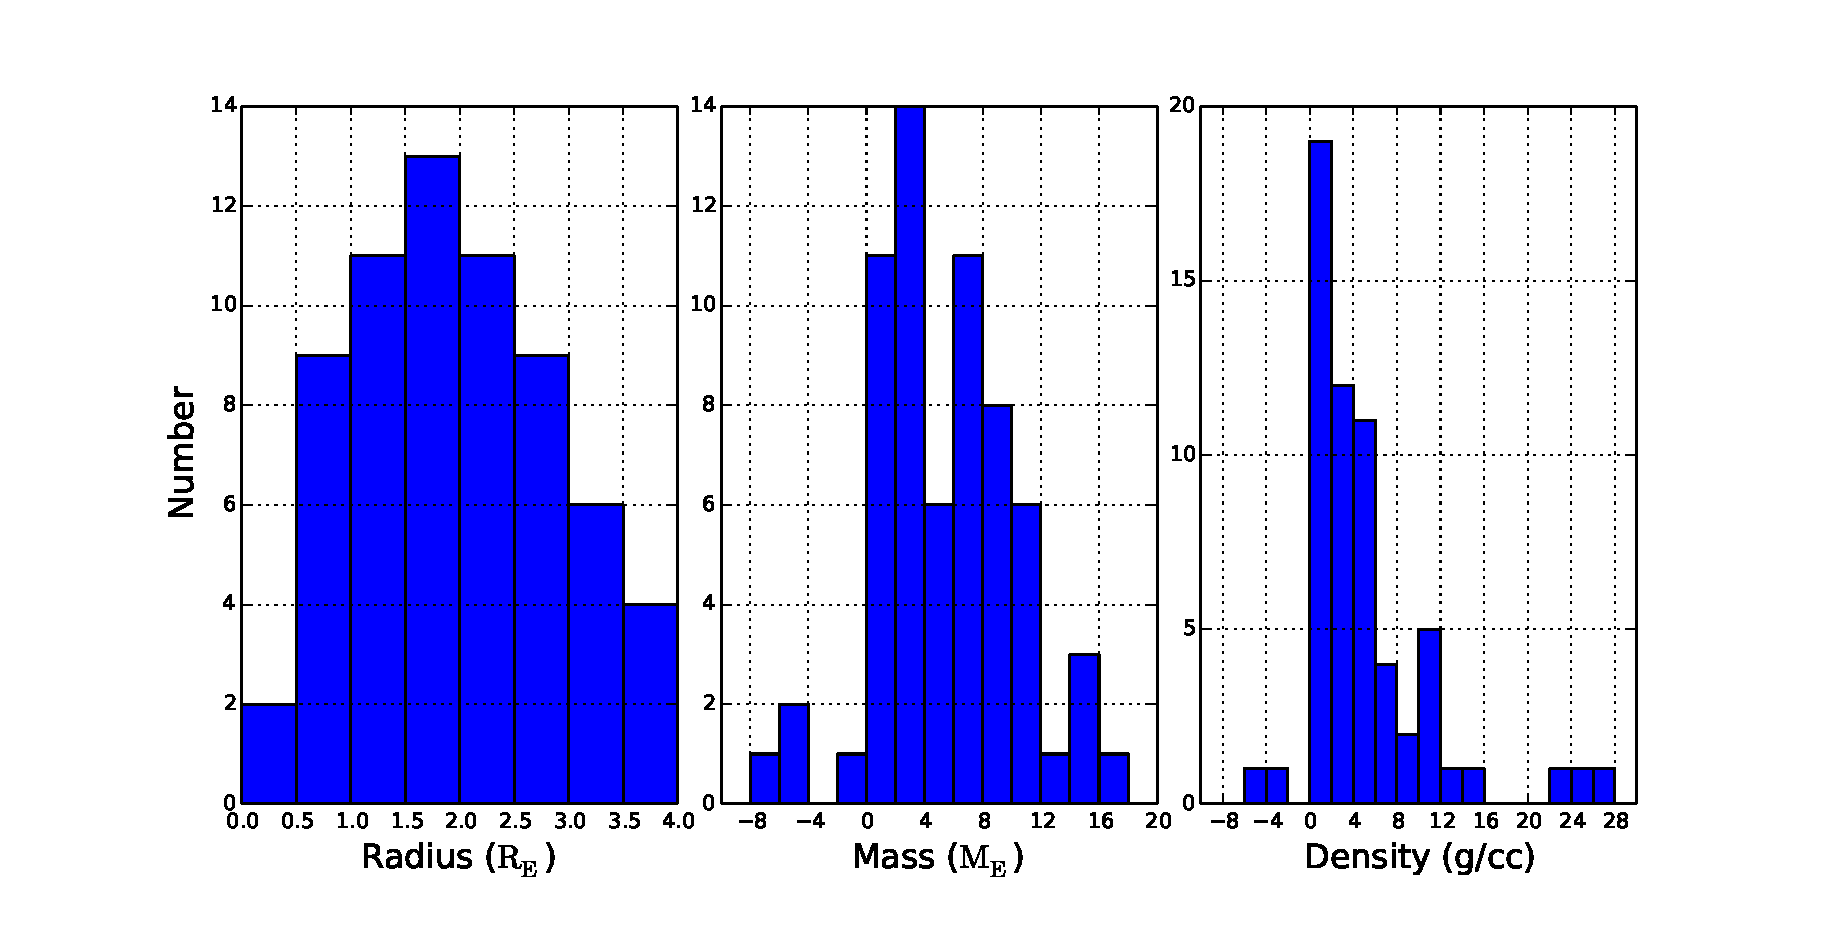
\includegraphics[width=6in]{histograms.eps} 
   \caption{\small Histograms of exoplanet radii, masses, and densities for the 60 exoplanets smaller then 4 Earth radii with measured masses or mass upper-limits.  Some mass and density outliers were excluded from these plots, but are included in Table 1 and the fits.}
\label{fig:histograms}
\end{figure*}

\begin{figure*}[htbp] %  figure placement: here, top, bottom, or page
   \centering
    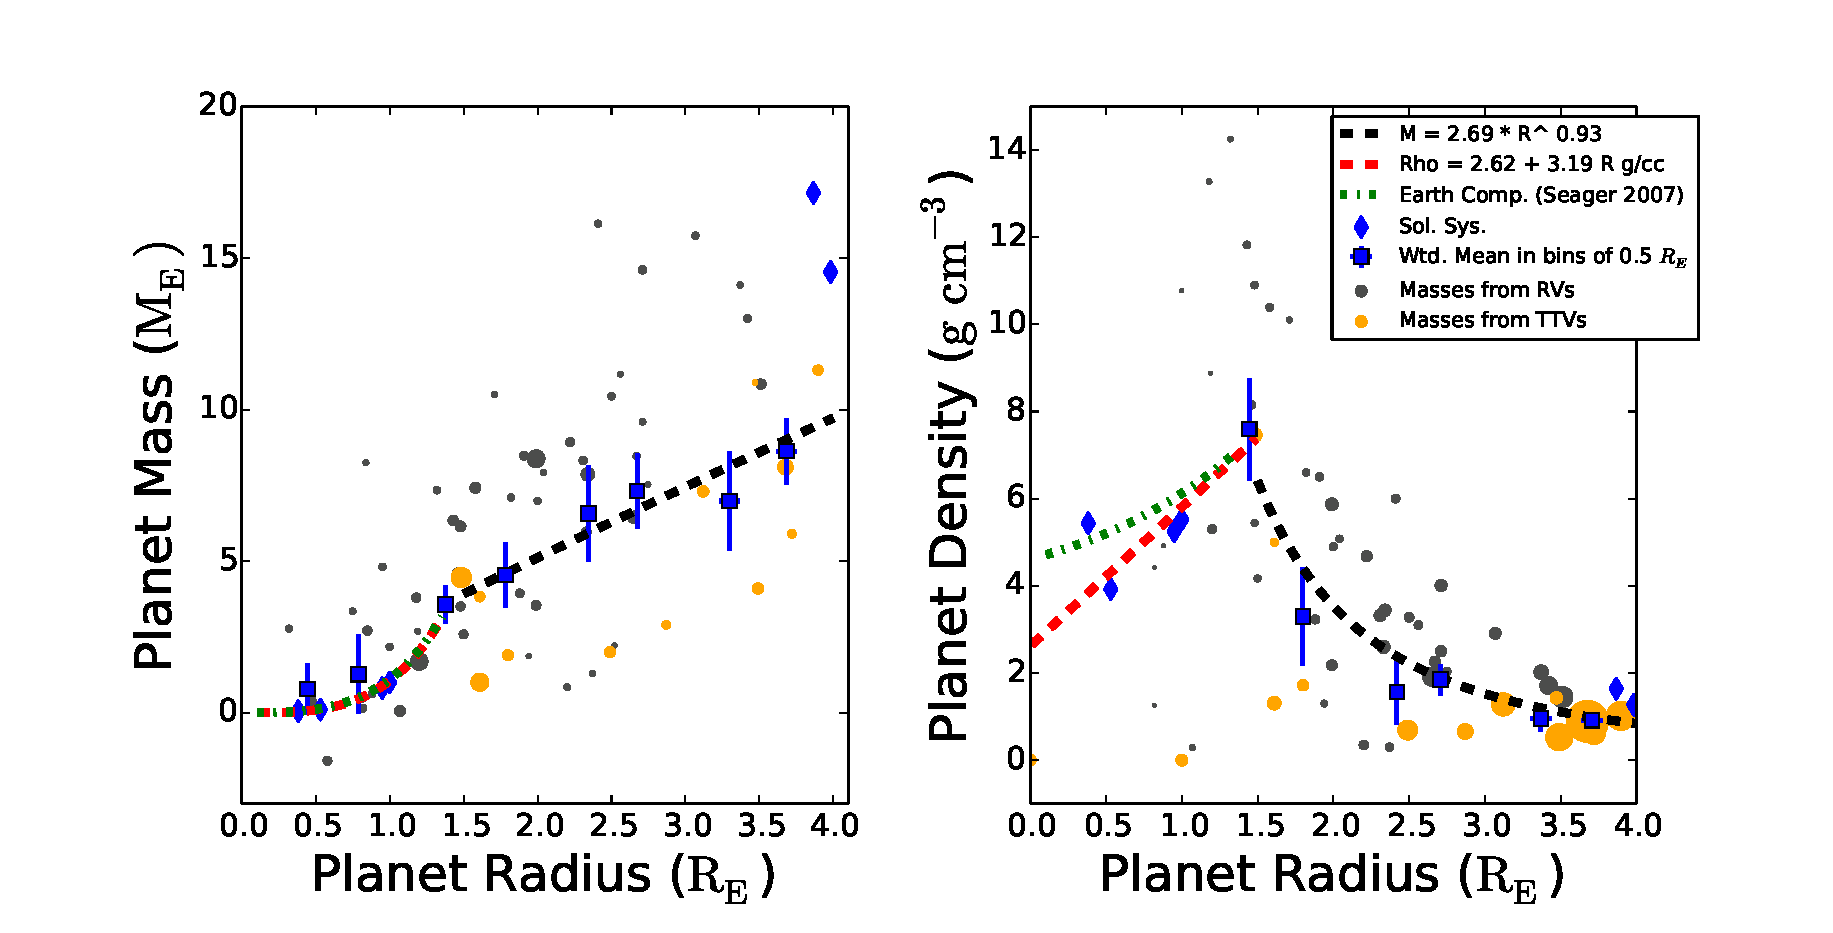
\includegraphics[width=6in]{mr_small.eps} 
   \caption{\small \textbf{Left:} Mass vs. radius for 60 exoplanets and 1$\sigma$ error bars.  Gray points  have RV-determined masses; orange points have TTV-determined masses.  The dashed lines correspond to the various empirical fits between planet mass and radius; see equations \ref{eqn:mr_plaw}, \ref{eqn:mr_linear}, and \ref{eqn:mr_rocky}.  The blue points are the weighted mean exoplanet mass in bins of $0.5 \rearth$, with error bars representing the uncertainty in the means.  The weighted means are to guide the eye only; they were not used in calculating the fits.  The magenta letters indicate solar system planets, which were used only in the cyan fit (equation \ref{eqn:mr_rocky}).  \textbf{Right:} Density vs. radius for 60 exoplanets and $1\sigma$ error bars.  Gray points  have RV-determined masses; orange points have TTV-determined masses.  Note that no exoplanets smaller than $1\rearth$ have densities determined to better than 6.5 \gcc.  The blue points are the weighted mean densities in bins of $0.5 \rearth$; these points are to guide the eye only and were not used in any of the fits.  The \citet{Seager2007} density-radius solution for Earth's composition (67.5\% Fe, 32.5\% MgSiO$_3$) is shown as the solid green line.  The dashed line corresponds to the polynomial empirical fit between planet density and radius; see equation \ref{eqn:dr_poly}.  Planets larger than 1.5 \rearth are less dense than Earth and much less dense than an Earth composition at that radius, indicating that planets satisfying $\rpl > 1.5 \rearth$ probably contain a significant fraction of volatiles by volume.  Some mass and density outliers were excluded from these plots, but are included in the fits.}
   \label{fig:rm_4}
\end{figure*}


\begin{figure*}[htbp] %  figure placement: here, top, bottom, or page
   \centering
    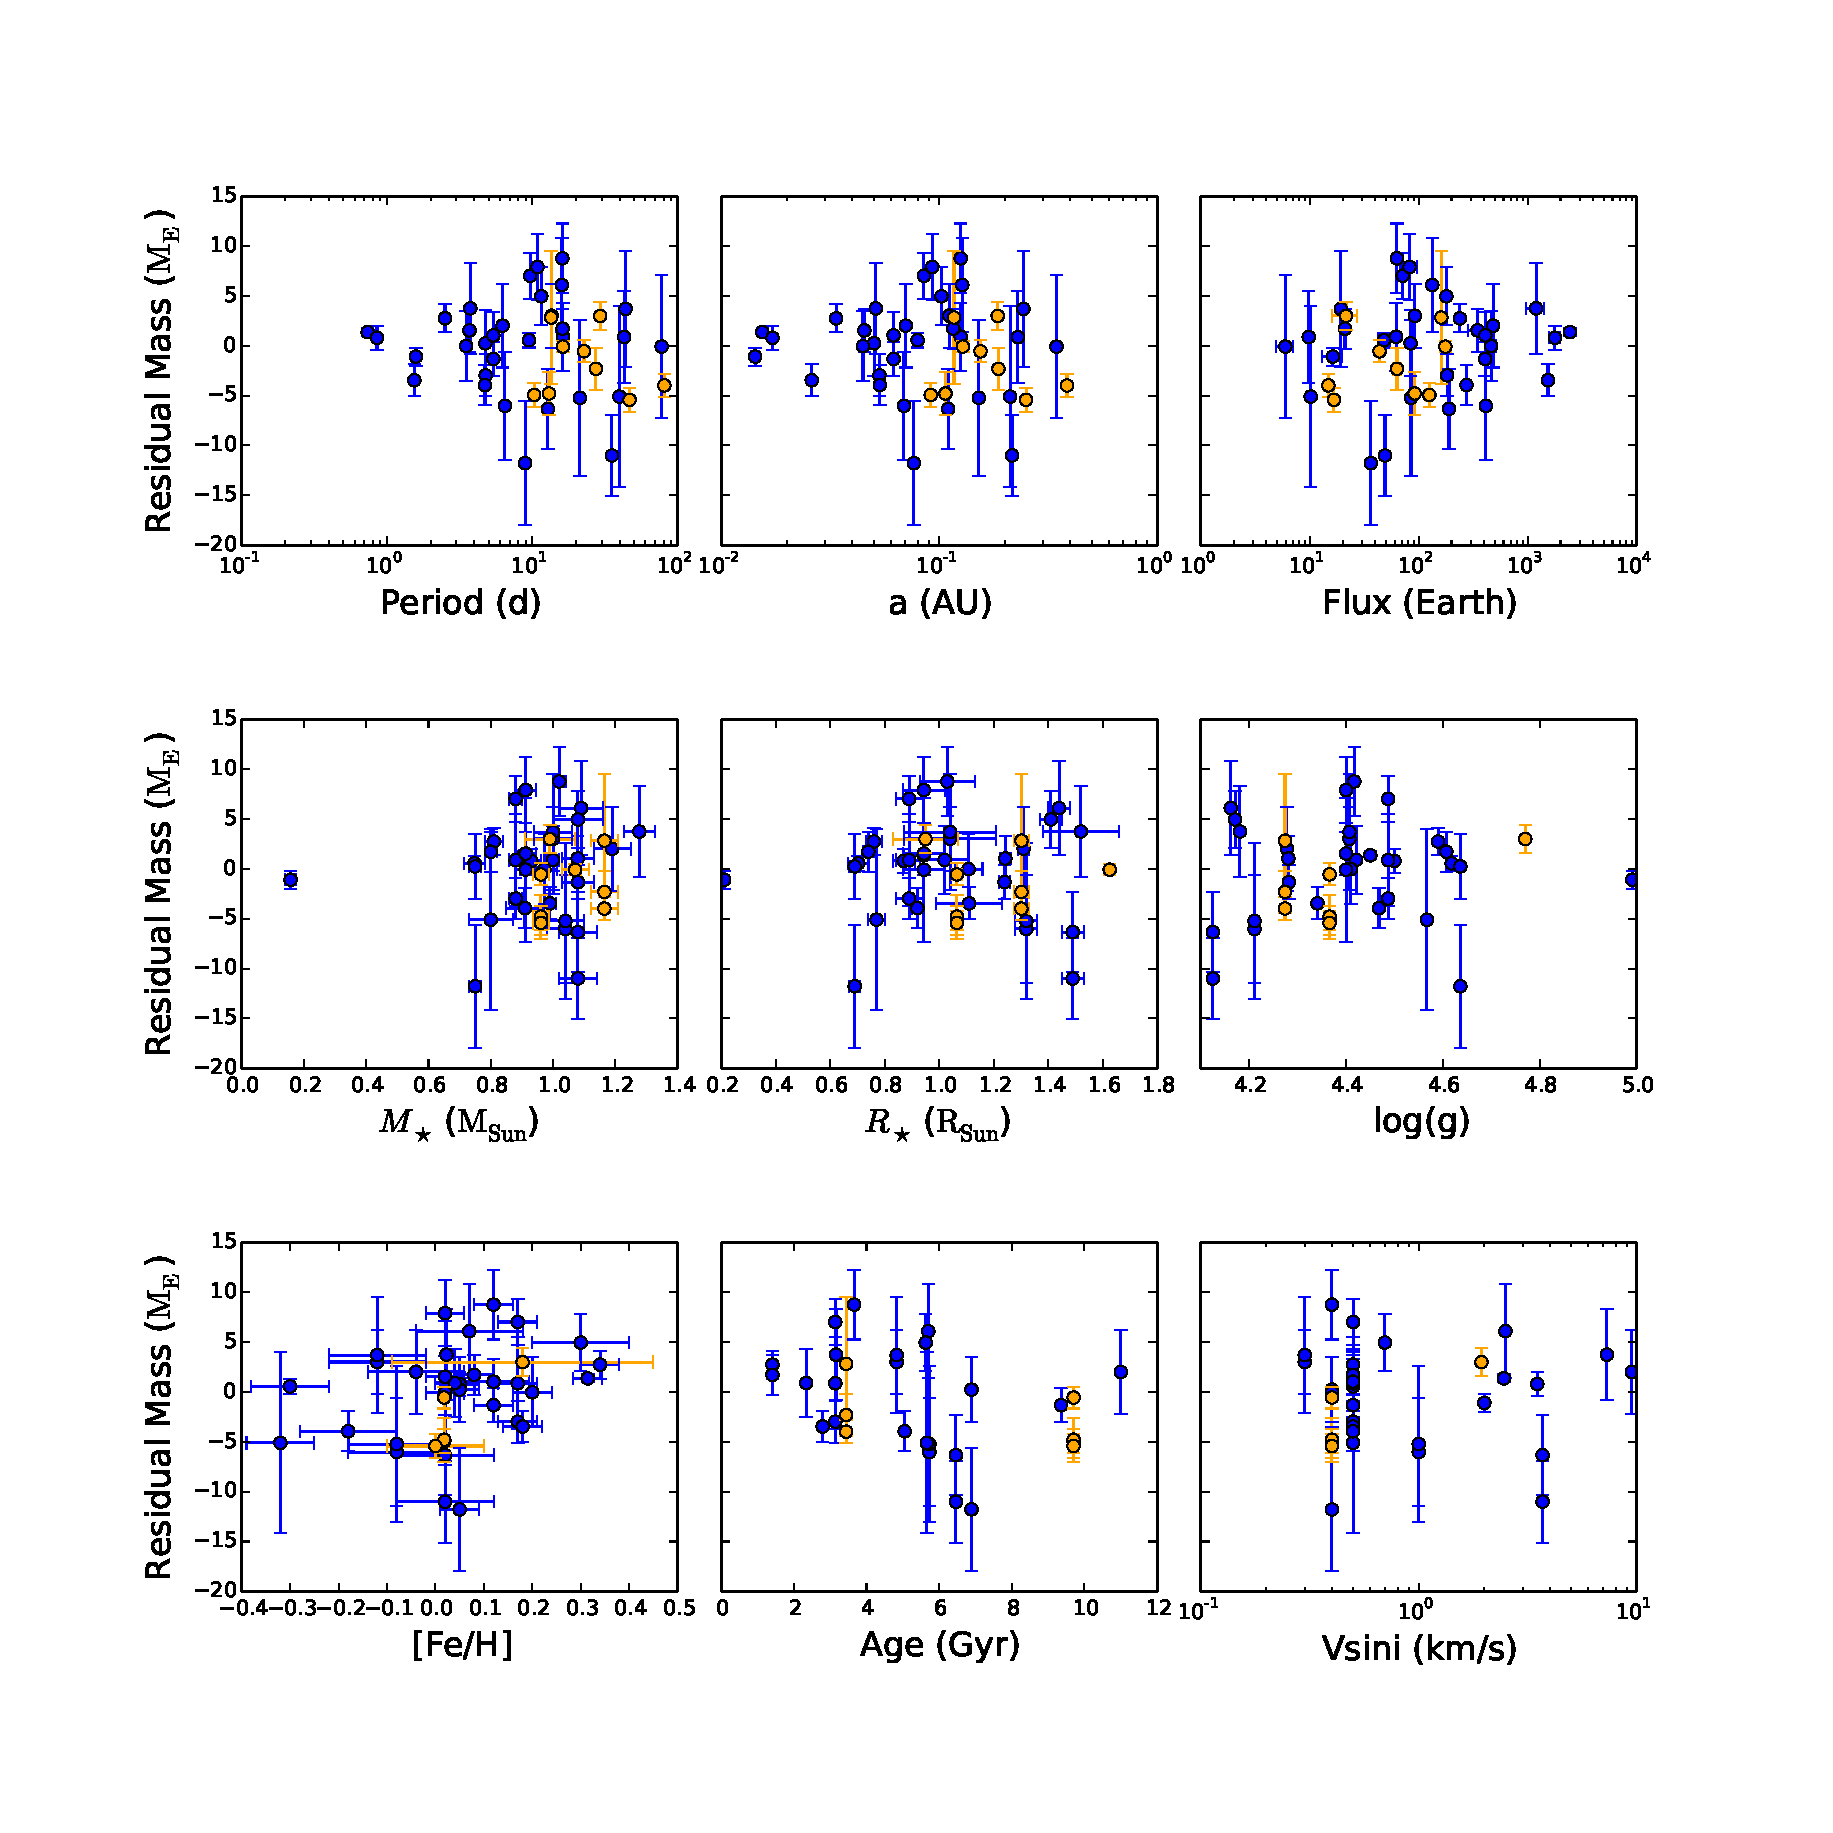
\includegraphics[width=6in]{mr_resids.eps} 
   \caption{\small Mass residuals (measured minus the mass predicted from equation \ref{eqn:mr_plaw}) versus (top left to bottom right): planet orbital period, planet semi-major axis, incident flux from the star on the planet, stellar mass, stellar radius, log surface gravity, log iron fraction (compared to solar), stellar age, and stellar velocity times the sine of the projected stellar inclination. Error bars are 1$\sigma$ uncertainties in mass measurements, and the orange points are residuals of the TTV-determined masses.  None of the residuals show a significant correlation.}
   \label{fig:resids}
\end{figure*}

%%%%%%%%%%%%% Bibliograpy %%%%%%%%%%%%%%%%%%%%%%%%%%%%%%%%
\clearpage

\begin{thebibliography}{32}
\expandafter\ifx\csname natexlab\endcsname\relax\def\natexlab#1{#1}\fi

\bibitem[{{Batalha} {et~al.}(2011){Batalha}, {Borucki}, {Bryson}, {Buchhave},
  {Caldwell}, {Christensen-Dalsgaard}, {Ciardi}, {Dunham}, {Fressin},
  {Gautier}, {Gilliland}, {Haas}, {Howell}, {Jenkins}, {Kjeldsen}, {Koch},
  {Latham}, {Lissauer}, {Marcy}, {Rowe}, {Sasselov}, {Seager}, {Steffen},
  {Torres}, {Basri}, {Brown}, {Charbonneau}, {Christiansen}, {Clarke},
  {Cochran}, {Dupree}, {Fabrycky}, {Fischer}, {Ford}, {Fortney}, {Girouard},
  {Holman}, {Johnson}, {Isaacson}, {Klaus}, {Machalek}, {Moorehead},
  {Morehead}, {Ragozzine}, {Tenenbaum}, {Twicken}, {Quinn}, {VanCleve},
  {Walkowicz}, {Welsh}, {Devore}, \& {Gould}}]{Batalha2011}
{Batalha}, N.~M., {Borucki}, W.~J., {Bryson}, S.~T., {et~al.} 2011, \apj, 729,
  27

\bibitem[{{Batalha} {et~al.}(2013){Batalha}, {Rowe}, {Bryson}, {Barclay},
  {Burke}, {Caldwell}, {Christiansen}, {Mullally}, {Thompson}, {Brown},
  {Dupree}, {Fabrycky}, {Ford}, {Fortney}, {Gilliland}, {Isaacson}, {Latham},
  {Marcy}, {Quinn}, {Ragozzine}, {Shporer}, {Borucki}, {Ciardi}, {Gautier},
  {Haas}, {Jenkins}, {Koch}, {Lissauer}, {Rapin}, {Basri}, {Boss}, {Buchhave},
  {Carter}, {Charbonneau}, {Christensen-Dalsgaard}, {Clarke}, {Cochran},
  {Demory}, {Desert}, {Devore}, {Doyle}, {Esquerdo}, {Everett}, {Fressin},
  {Geary}, {Girouard}, {Gould}, {Hall}, {Holman}, {Howard}, {Howell},
  {Ibrahim}, {Kinemuchi}, {Kjeldsen}, {Klaus}, {Li}, {Lucas}, {Meibom},
  {Morris}, {Pr{\v s}a}, {Quintana}, {Sanderfer}, {Sasselov}, {Seader},
  {Smith}, {Steffen}, {Still}, {Stumpe}, {Tarter}, {Tenenbaum}, {Torres},
  {Twicken}, {Uddin}, {Van Cleve}, {Walkowicz}, \& {Welsh}}]{Batalha2013}
{Batalha}, N.~M., {Rowe}, J.~F., {Bryson}, S.~T., {et~al.} 2013, \apjs, 204, 24

\bibitem[{{Borucki} {et~al.}(2011){Borucki}, {Koch}, {Basri}, {Batalha},
  {Brown}, {Bryson}, {Caldwell}, {Christensen-Dalsgaard}, {Cochran}, {DeVore},
  {Dunham}, {Gautier}, {Geary}, {Gilliland}, {Gould}, {Howell}, {Jenkins},
  {Latham}, {Lissauer}, {Marcy}, {Rowe}, {Sasselov}, {Boss}, {Charbonneau},
  {Ciardi}, {Doyle}, {Dupree}, {Ford}, {Fortney}, {Holman}, {Seager},
  {Steffen}, {Tarter}, {Welsh}, {Allen}, {Buchhave}, {Christiansen}, {Clarke},
  {Das}, {D{\'e}sert}, {Endl}, {Fabrycky}, {Fressin}, {Haas}, {Horch},
  {Howard}, {Isaacson}, {Kjeldsen}, {Kolodziejczak}, {Kulesa}, {Li}, {Lucas},
  {Machalek}, {McCarthy}, {MacQueen}, {Meibom}, {Miquel}, {Prsa}, {Quinn},
  {Quintana}, {Ragozzine}, {Sherry}, {Shporer}, {Tenenbaum}, {Torres},
  {Twicken}, {Van Cleve}, {Walkowicz}, {Witteborn}, \& {Still}}]{Borucki2011}
{Borucki}, W.~J., {Koch}, D.~G., {Basri}, G., {et~al.} 2011, \apj, 736, 19

\bibitem[{{Buchhave} {et~al.}(2012){Buchhave}, {Latham}, {Johansen},
  {Bizzarro}, {Torres}, {Rowe}, {Batalha}, {Borucki}, {Brugamyer}, {Caldwell},
  {Bryson}, {Ciardi}, {Cochran}, {Endl}, {Esquerdo}, {Ford}, {Geary},
  {Gilliland}, {Hansen}, {Isaacson}, {Laird}, {Lucas}, {Marcy}, {Morse},
  {Robertson}, {Shporer}, {Stefanik}, {Still}, \& {Quinn}}]{Buchhave2012}
{Buchhave}, L.~A., {Latham}, D.~W., {Johansen}, A., {et~al.} 2012, \nat, 486,
  375

\bibitem[{{Carter} {et~al.}(2011){Carter}, {Winn}, {Holman}, {Fabrycky},
  {Berta}, {Burke}, \& {Nutzman}}]{Carter2011}
{Carter}, J.~A., {Winn}, J.~N., {Holman}, M.~J., {et~al.} 2011, \apj, 730, 82

\bibitem[{{Carter} {et~al.}(2012){Carter}, {Agol}, {Chaplin}, {Basu},
  {Bedding}, {Buchhave}, {Christensen-Dalsgaard}, {Deck}, {Elsworth},
  {Fabrycky}, {Ford}, {Fortney}, {Hale}, {Handberg}, {Hekker}, {Holman},
  {Huber}, {Karoff}, {Kawaler}, {Kjeldsen}, {Lissauer}, {Lopez}, {Lund},
  {Lundkvist}, {Metcalfe}, {Miglio}, {Rogers}, {Stello}, {Borucki}, {Bryson},
  {Christiansen}, {Cochran}, {Geary}, {Gilliland}, {Haas}, {Hall}, {Howard},
  {Jenkins}, {Klaus}, {Koch}, {Latham}, {MacQueen}, {Sasselov}, {Steffen},
  {Twicken}, \& {Winn}}]{Carter2012}
{Carter}, J.~A., {Agol}, E., {Chaplin}, W.~J., {et~al.} 2012, Science, 337, 556

\bibitem[{{Charbonneau} {et~al.}(2009){Charbonneau}, {Berta}, {Irwin}, {Burke},
  {Nutzman}, {Buchhave}, {Lovis}, {Bonfils}, {Latham}, {Udry}, {Murray-Clay},
  {Holman}, {Falco}, {Winn}, {Queloz}, {Pepe}, {Mayor}, {Delfosse}, \&
  {Forveille}}]{Charbonneau2009}
{Charbonneau}, D., {Berta}, Z.~K., {Irwin}, J., {et~al.} 2009, \nat, 462, 891

\bibitem[{{Cochran} {et~al.}(2011){Cochran}, {Fabrycky}, {Torres}, {Fressin},
  {D{\'e}sert}, {Ragozzine}, {Sasselov}, {Fortney}, {Rowe}, {Brugamyer},
  {Bryson}, {Carter}, {Ciardi}, {Howell}, {Steffen}, {Borucki}, {Koch}, {Winn},
  {Welsh}, {Uddin}, {Tenenbaum}, {Still}, {Seager}, {Quinn}, {Mullally},
  {Miller}, {Marcy}, {MacQueen}, {Lucas}, {Lissauer}, {Latham}, {Knutson},
  {Kinemuchi}, {Johnson}, {Jenkins}, {Isaacson}, {Howard}, {Horch}, {Holman},
  {Henze}, {Haas}, {Gilliland}, {Gautier}, {Ford}, {Fischer}, {Everett},
  {Endl}, {Demory}, {Deming}, {Charbonneau}, {Caldwell}, {Buchhave}, {Brown},
  \& {Batalha}}]{Cochran2011}
{Cochran}, W.~D., {Fabrycky}, D.~C., {Torres}, G., {et~al.} 2011, \apjs, 197, 7

\bibitem[{{Dragomir} {et~al.}(2013{\natexlab{a}}){Dragomir}, {Matthews},
  {Winn}, {Rowe}, \& {MOST Science Team}}]{Dragomir2013b}
{Dragomir}, D., {Matthews}, J.~M., {Winn}, J.~N., {Rowe}, J.~F., \& {MOST
  Science Team}. 2013{\natexlab{a}}, ArXiv e-prints

\bibitem[{{Dragomir} {et~al.}(2013{\natexlab{b}}){Dragomir}, {Matthews},
  {Eastman}, {Cameron}, {Howard}, {Guenther}, {Kuschnig}, {Moffat}, {Rowe},
  {Rucinski}, {Sasselov}, \& {Weiss}}]{Dragomir2013}
{Dragomir}, D., {Matthews}, J.~M., {Eastman}, J.~D., {et~al.}
  2013{\natexlab{b}}, \apjl, 772, L2

\bibitem[{{Endl} {et~al.}(2012){Endl}, {Robertson}, {Cochran}, {MacQueen},
  {Brugamyer}, {Caldwell}, {Wittenmyer}, {Barnes}, \& {Gullikson}}]{Endl2012}
{Endl}, M., {Robertson}, P., {Cochran}, W.~D., {et~al.} 2012, \apj, 759, 19

\bibitem[{{Enoch} {et~al.}(2012){Enoch}, {Collier Cameron}, \&
  {Horne}}]{Enoch2012}
{Enoch}, B., {Collier Cameron}, A., \& {Horne}, K. 2012, \aap, 540, A99

\bibitem[{{Gautier} {et~al.}(2012){Gautier}, {Charbonneau}, {Rowe}, {Marcy},
  {Isaacson}, {Torres}, {Fressin}, {Rogers}, {D{\'e}sert}, {Buchhave},
  {Latham}, {Quinn}, {Ciardi}, {Fabrycky}, {Ford}, {Gilliland}, {Walkowicz},
  {Bryson}, {Cochran}, {Endl}, {Fischer}, {Howell}, {Horch}, {Barclay},
  {Batalha}, {Borucki}, {Christiansen}, {Geary}, {Henze}, {Holman}, {Ibrahim},
  {Jenkins}, {Kinemuchi}, {Koch}, {Lissauer}, {Sanderfer}, {Sasselov},
  {Seager}, {Silverio}, {Smith}, {Still}, {Stumpe}, {Tenenbaum}, \& {Van
  Cleve}}]{Gautier2012}
{Gautier}, III, T.~N., {Charbonneau}, D., {Rowe}, J.~F., {et~al.} 2012, \apj,
  749, 15

\bibitem[{{Gilliland} {et~al.}(2013){Gilliland}, {Marcy}, {Rowe}, {Rogers},
  {Torres}, {Fressin}, {Lopez}, {Buchhave}, {Christensen-Dalsgaard},
  {D{\'e}sert}, {Henze}, {Isaacson}, {Jenkins}, {Lissauer}, {Chaplin}, {Basu},
  {Metcalfe}, {Elsworth}, {Handberg}, {Hekker}, {Huber}, {Karoff}, {Kjeldsen},
  {Lund}, {Lundkvist}, {Miglio}, {Charbonneau}, {Ford}, {Fortney}, {Haas},
  {Howard}, {Howell}, {Ragozzine}, \& {Thompson}}]{Gilliland2013}
{Gilliland}, R.~L., {Marcy}, G.~W., {Rowe}, J.~F., {et~al.} 2013, \apj, 766, 40

\bibitem[{{Hatzes} {et~al.}(2011){Hatzes}, {Fridlund}, {Nachmani}, {Mazeh},
  {Valencia}, {H{\'e}brard}, {Carone}, {P{\"a}tzold}, {Udry}, {Bouchy},
  {Deleuil}, {Moutou}, {Barge}, {Bord{\'e}}, {Deeg}, {Tingley}, {Dvorak},
  {Gandolfi}, {Ferraz-Mello}, {Wuchterl}, {Guenther}, {Guillot}, {Rauer},
  {Erikson}, {Cabrera}, {Csizmadia}, {L{\'e}ger}, {Lammer}, {Weingrill},
  {Queloz}, {Alonso}, {Rouan}, \& {Schneider}}]{Hatzes2011}
{Hatzes}, A.~P., {Fridlund}, M., {Nachmani}, G., {et~al.} 2011, \apj, 743, 75

\bibitem[{Howard {et~al.}(2011)Howard, Johnson, Marcy, Fischer, Wright, Henry,
  Isaacson, Valenti, Anderson, \& Piskunov}]{Howard2011}
Howard, A.~W., Johnson, J.~A., Marcy, G.~W., {et~al.} 2011, The Astrophysical
  Journal, 726, 73

\bibitem[{{Howard} {et~al.}(2013){Howard}, {Sanchis-Ojeda}, {Marcy}, {Johnson},
  {Winn}, {Isaacson}, {Fischer}, {Fulton}, {Sinukoff}, \&
  {Fortney}}]{Howard2013arxiv}
{Howard}, A.~W., {Sanchis-Ojeda}, R., {Marcy}, G.~W., {et~al.} 2013, ArXiv
  e-prints

\bibitem[{{Kane} \& {Gelino}(2012)}]{Kane2012}
{Kane}, S.~R., \& {Gelino}, D.~M. 2012, \pasp, 124, 323

\bibitem[{{L{\'e}ger} {et~al.}(2009){L{\'e}ger}, {Rouan}, {Schneider}, {Barge},
  {Fridlund}, {Samuel}, {Ollivier}, {Guenther}, {Deleuil}, {Deeg}, {Auvergne},
  {Alonso}, {Aigrain}, {Alapini}, {Almenara}, {Baglin}, {Barbieri}, {Bruntt},
  {Bord{\'e}}, {Bouchy}, {Cabrera}, {Catala}, {Carone}, {Carpano}, {Csizmadia},
  {Dvorak}, {Erikson}, {Ferraz-Mello}, {Foing}, {Fressin}, {Gandolfi},
  {Gillon}, {Gondoin}, {Grasset}, {Guillot}, {Hatzes}, {H{\'e}brard}, {Jorda},
  {Lammer}, {Llebaria}, {Loeillet}, {Mayor}, {Mazeh}, {Moutou}, {P{\"a}tzold},
  {Pont}, {Queloz}, {Rauer}, {Renner}, {Samadi}, {Shporer}, {Sotin}, {Tingley},
  {Wuchterl}, {Adda}, {Agogu}, {Appourchaux}, {Ballans}, {Baron}, {Beaufort},
  {Bellenger}, {Berlin}, {Bernardi}, {Blouin}, {Baudin}, {Bodin}, {Boisnard},
  {Boit}, {Bonneau}, {Borzeix}, {Briet}, {Buey}, {Butler}, {Cailleau},
  {Cautain}, {Chabaud}, {Chaintreuil}, {Chiavassa}, {Costes}, {Cuna Parrho},
  {de Oliveira Fialho}, {Decaudin}, {Defise}, {Djalal}, {Epstein}, {Exil},
  {Faur{\'e}}, {Fenouillet}, {Gaboriaud}, {Gallic}, {Gamet}, {Gavalda},
  {Grolleau}, {Gruneisen}, {Gueguen}, {Guis}, {Guivarc'h}, {Guterman},
  {Hallouard}, {Hasiba}, {Heuripeau}, {Huntzinger}, {Hustaix}, {Imad},
  {Imbert}, {Johlander}, {Jouret}, {Journoud}, {Karioty}, {Kerjean},
  {Lafaille}, {Lafond}, {Lam-Trong}, {Landiech}, {Lapeyrere}, {Larqu{\'e}},
  {Laudet}, {Lautier}, {Lecann}, {Lefevre}, {Leruyet}, {Levacher}, {Magnan},
  {Mazy}, {Mertens}, {Mesnager}, {Meunier}, {Michel}, {Monjoin}, {Naudet},
  {Nguyen-Kim}, {Orcesi}, {Ottacher}, {Perez}, {Peter}, {Plasson}, {Plesseria},
  {Pontet}, {Pradines}, {Quentin}, {Reynaud}, {Rolland}, {Rollenhagen},
  {Romagnan}, {Russ}, {Schmidt}, {Schwartz}, {Sebbag}, {Sedes}, {Smit},
  {Steller}, {Sunter}, {Surace}, {Tello}, {Tiph{\`e}ne}, {Toulouse}, {Ulmer},
  {Vandermarcq}, {Vergnault}, {Vuillemin}, \& {Zanatta}}]{Leger2009}
{L{\'e}ger}, A., {Rouan}, D., {Schneider}, J., {et~al.} 2009, \aap, 506, 287

\bibitem[{{Lissauer} {et~al.}(2011){Lissauer}, {Fabrycky}, {Ford}, {Borucki},
  {Fressin}, {Marcy}, {Orosz}, {Rowe}, {Torres}, {Welsh}, {Batalha}, {Bryson},
  {Buchhave}, {Caldwell}, {Carter}, {Charbonneau}, {Christiansen}, {Cochran},
  {Desert}, {Dunham}, {Fanelli}, {Fortney}, {Gautier}, {Geary}, {Gilliland},
  {Haas}, {Hall}, {Holman}, {Koch}, {Latham}, {Lopez}, {McCauliff}, {Miller},
  {Morehead}, {Quintana}, {Ragozzine}, {Sasselov}, {Short}, \&
  {Steffen}}]{Lissauer2011}
{Lissauer}, J.~J., {Fabrycky}, D.~C., {Ford}, E.~B., {et~al.} 2011, \nat, 470,
  53

\bibitem[{{Lissauer} {et~al.}(2013){Lissauer}, {Jontof-Hutter}, {Rowe},
  {Fabrycky}, {Lopez}, {Agol}, {Marcy}, {Deck}, {Fischer}, {Fortney}, {Howell},
  {Isaacson}, {Jenkins}, {Kolbl}, {Sasselov}, {Short}, \&
  {Welsh}}]{Lissauer2013}
{Lissauer}, J.~J., {Jontof-Hutter}, D., {Rowe}, J.~F., {et~al.} 2013, \apj,
  770, 131

\bibitem[{{Lopez} {et~al.}(2012){Lopez}, {Fortney}, \& {Miller}}]{Lopez2012}
{Lopez}, E.~D., {Fortney}, J.~J., \& {Miller}, N.~K. 2012, ArXiv e-prints

\bibitem[{{Marcy} {et~al.}(2013){Marcy}, {Isaacson}, \& {Rowe}}]{Marcy2013}
{Marcy}, G.~W., {Isaacson}, H., \& {Rowe}, J.~F. 2013, in prep.

\bibitem[{{McArthur} {et~al.}(2004){McArthur}, {Endl}, {Cochran}, {Benedict},
  {Fischer}, {Marcy}, {Butler}, {Naef}, {Mayor}, {Queloz}, {Udry}, \&
  {Harrison}}]{McArthur2004}
{McArthur}, B.~E., {Endl}, M., {Cochran}, W.~D., {et~al.} 2004, \apjl, 614, L81

\bibitem[{{Petigura} {et~al.}(2013){Petigura}, {Marcy}, \&
  {Howard}}]{Petigura2013a}
{Petigura}, E.~A., {Marcy}, G.~W., \& {Howard}, A.~W. 2013, \apj, 770, 69

\bibitem[{{Queloz} {et~al.}(2009){Queloz}, {Bouchy}, {Moutou}, {Hatzes},
  {H{\'e}brard}, {Alonso}, {Auvergne}, {Baglin}, {Barbieri}, {Barge}, {Benz},
  {Bord{\'e}}, {Deeg}, {Deleuil}, {Dvorak}, {Erikson}, {Ferraz Mello},
  {Fridlund}, {Gandolfi}, {Gillon}, {Guenther}, {Guillot}, {Jorda}, {Hartmann},
  {Lammer}, {L{\'e}ger}, {Llebaria}, {Lovis}, {Magain}, {Mayor}, {Mazeh},
  {Ollivier}, {P{\"a}tzold}, {Pepe}, {Rauer}, {Rouan}, {Schneider},
  {Segransan}, {Udry}, \& {Wuchterl}}]{Queloz2009}
{Queloz}, D., {Bouchy}, F., {Moutou}, C., {et~al.} 2009, \aap, 506, 303

\bibitem[{{Sanchis-Ojeda} {et~al.}(2013){Sanchis-Ojeda}, {Rappaport}, {Winn},
  {Levine}, {Kotson}, {Latham}, \& {Buchhave}}]{Sanchis-Ojeda2013}
{Sanchis-Ojeda}, R., {Rappaport}, S., {Winn}, J.~N., {et~al.} 2013, \apj, 774,
  54

\bibitem[{{Sanchis-Ojeda} {et~al.}(2012){Sanchis-Ojeda}, {Fabrycky}, {Winn},
  {Barclay}, {Clarke}, {Ford}, {Fortney}, {Geary}, {Holman}, {Howard},
  {Jenkins}, {Koch}, {Lissauer}, {Marcy}, {Mullally}, {Ragozzine}, {Seader},
  {Still}, \& {Thompson}}]{Sanchis-Ojeda2012}
{Sanchis-Ojeda}, R., {Fabrycky}, D.~C., {Winn}, J.~N., {et~al.} 2012, \nat,
  487, 449

\bibitem[{{Seager} {et~al.}(2007){Seager}, {Kuchner}, {Hier-Majumder}, \&
  {Militzer}}]{Seager2007}
{Seager}, S., {Kuchner}, M., {Hier-Majumder}, C.~A., \& {Militzer}, B. 2007,
  \apj, 669, 1279

\bibitem[{{Torres} {et~al.}(2012){Torres}, {Fischer}, {Sozzetti}, {Buchhave},
  {Winn}, {Holman}, \& {Carter}}]{Torres2012}
{Torres}, G., {Fischer}, D.~A., {Sozzetti}, A., {et~al.} 2012, \apj, 757, 161

\bibitem[{{Weiss} {et~al.}(2013){Weiss}, {Marcy}, {Rowe}, {Howard}, {Isaacson},
  {Fortney}, {Miller}, {Demory}, {Fischer}, {Adams}, {Dupree}, {Howell},
  {Kolbl}, {Johnson}, {Horch}, {Everett}, {Fabrycky}, \& {Seager}}]{Weiss2013}
{Weiss}, L.~M., {Marcy}, G.~W., {Rowe}, J.~F., {et~al.} 2013, \apj, 768, 14

\bibitem[{{Wu} \& {Lithwick}(2013)}]{WL2013}
{Wu}, Y., \& {Lithwick}, Y. 2013, \apj, 772, 74

\end{thebibliography}

\bibliographystyle{apj}

\end{document}  